% The contents of this file is 
% Copyright (c) 2009-  Charles R. Severance, All Righs Reserved

\chapter{Bases de datos y SQL}

\section{¿Qué es una base de datos?}
\index{base de datos}

Una {\bf base de datos} es un archivo que está organizado para almacenar datos.
La mayoría de las bases de datos están organizadas como diccionarios, en el sentido
de que realizan mapeados entre claves y valores. La diferencia más importante
es que la base de datos se encuentra en el disco (u otro almacenamiento permanente),
de modo que su contenido se conserva después de que el programa finaliza. Gracias a que la base de
datos se guarda en un almacenamiento permanente, puede almacenar muchos más datos que
un diccionario, que está limitado al tamaño de la memoria
que tenga el ordenador.

\index{base de datos!índices}
Como un diccionario, el software de una base de datos está diseñado para conseguir que
la inserción y acceso a los datos sean muy rápidos, incluso para grandes
cantidades de datos. Este software mantiene su rendimiento mediante la
construcción de {\bf índices}, como datos añadidos a la base de datos
que permiten al ordenador saltar rápidamente hasta una entrada
concreta.

Existen muchos sistemas de bases de datos diferentes, que se utilizan para una
amplia variedad de propósitos. Algunos de ellos son: Oracle, MySQL, Microsoft SQL Server,
PostgrSQL, y SQLite. En este libro nos centraremos en SQLite, ya que
se trata de una base de datos muy habitual y ya viene integrada dentro de Python.
SQLite está diseñada para ser \emph{incrustada} dentro de otras aplicaciones
de modo que proporcione soporte para bases de datos dentro de la aplicación. Por ejemplo,
el navegador Firefox es uno de los que utilizan la base de datos SQLite internamente,
al igual que muchos otros productos.

\url{http://sqlite.org/}

SQLite es muy adecuado para ciertos problemas de manipulación de datos que nos
encontramos en informática, como en la aplicación de rastreo de Twitter que
hemos descrito en el capítulo anterior.

\section{Conceptos sobre bases de datos}

Cuando se ve por primera vez una base de datos, se asemeja a una
hoja de cálculo con múltiples hojas. Las estructuras de datos primarias
en una base de datos son:
{\bf tablas}, {\bf filas}, y {\bf columnas}.  

\beforefig
\centerline{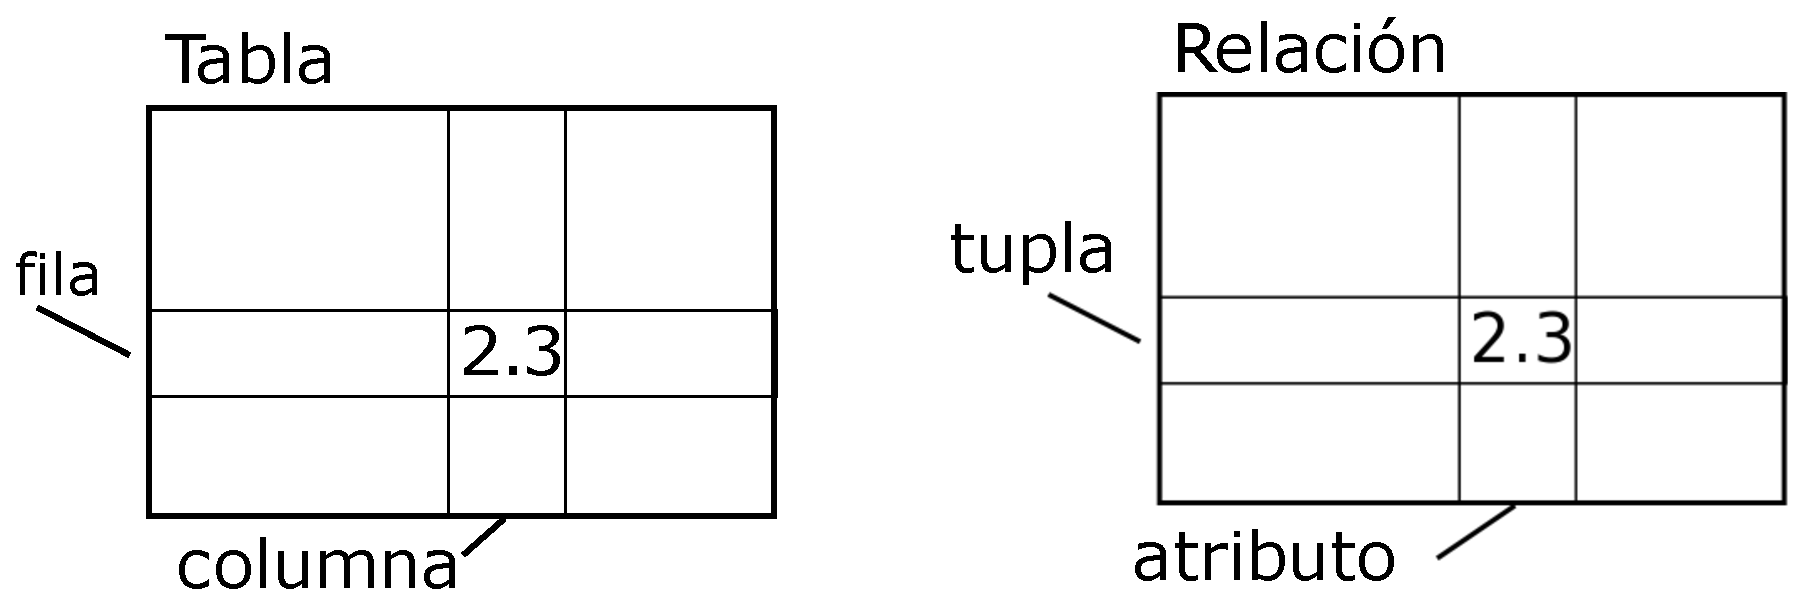
\includegraphics[height=1.50in]{figs2/relational.eps}}
\afterfig

En las descripciones técnicas de las bases de datos relacionales, los conceptos de
tabla, fila y columna reciben los nombres más formales
de {\bf relación}, {\bf tupla}, y {\bf atributo} respectivamente.
Nosotros a lo largo de este capítulo usaremos los términos menos formales.

\section{Add-on de Firefox para gestión de SQLite}

A pesar de que en este capítulo nos centraremos en el uso de Python para trabajar con datos
en archivos de bases de datos SQLite, hay muchas operaciones que pueden realizarse
de forma más eficaz usando un add-on para Firefox llamado {\bf SQLite
Database Manager}, que se puede descargar libremente desde:

\url{https://addons.mozilla.org/en-us/firefox/addon/sqlite-manager/}

Utilizando el navegador se pueden crear tablas con facilidad, insertar y editar datos
o ejecutar consultas SQL sencillas sobre la base de datos.

En cierto sentido, el gestor de base de datos es parecido a un editor de texto
que trabaja con archivos de texto. Cuando quieres realizar uno o
dos cambios en un archivo de texto, lo más sencillo es abrirlo en
un editor de texto y realizar los cambios que quieres. Cuando debes realizar
muchas modificaciones en el archivo, a menudo
habrá que escribir un programa en Python sencillo. El mismo enfoque
se puede aplicar al trabajo con bases de datos. Se realizarán las
operaciones más sencillas en el gestor de bases de datos, y para otras más complejas
será más conveniente usar Python.

\section{Creación de una tabla en una base de datos}

Las bases de datos necesitan una estructura más definida que las listas
o diccionarios de Python\footnote{SQLite en realidad permite cierta
flexibilidad respecto al tipo de datos que se almacenan en cada columna,
pero en este capítulo nosotros vamos a mantener los tipos de datos estrictos
para que los conceptos que aprendamos puedan ser igualmente aplicados a otras
bases de datos como MySQL.}.

Cuando se crea una {\bf tabla}, se debe
indicar de antemano a la base de datos los nombres de cada una de las
{\bf columnas} de la tabla y el tipo de datos que se van a
almacenar en cada {\bf columna}. Cuando el software de la base de datos
conoce el tipo de datos de cada columna, puede elegir el modo más
eficiente de almacenar y buscar en ellas, de acuerdo al tipo de
datos guardados.

Puedes revisar los distintos tipos de datos soportados por SQLite
en la siguiente dirección:

\url{http://www.sqlite.org/datatypes.html}

El tener que definir de antemano una estructura para los datos puede parecer incómodo
al principio, pero la recompensa consiste en obtener un acceso rápido a los datos,
incluso cuando la base de datos contiene una gran cantidad de ellos.

El código para crear un archivo de base de datos y una tabla
llamada {\tt Canciones} con dos columnas en la
base de datos es el siguiente:

\index{sqlite3, módulo}
\index{módulo!sqlite3}
\beforeverb
\begin{verbatim}
import sqlite3

conn = sqlite3.connect('musica.sqlite3')
cur = conn.cursor()

cur.execute('DROP TABLE IF EXISTS Canciones ')
cur.execute('CREATE TABLE Canciones (titulo TEXT, reproducciones INTEGER)')

conn.close()
\end{verbatim}
\afterverb
%
\index{connect, función}
\index{función!connect}
\index{cursor, función}
\index{función!cursor}
La operación {\tt connect} realiza una ``conexión'' con la base de datos
almacenada en el archivo {\tt musica.sqlite3} del directorio actual. Si
el archivo no existe, se creará nuevo. La razón de que se le
llame una ``conexión'' es que a veces la base de datos se almacena en
un ``servidor de bases de datos'', distinto del servidor en el cual está
funcionando nuestra aplicación. En nuestros ejemplos, dado que son sencillos,
la base de datos será simplemente un archivo local en el mismo directorio
en el que está funcionando el código de Python.

Un {\bf cursor} es como un manejador de fichero, y se puede usar para realizar
operaciones en los datos almacenados en la base de datos. La llamada a
{\tt cursor()} es muy parecida conceptualmente a la llamada a
{\tt open()} cuando se está tratando con ficheros de texto.

\beforefig
\centerline{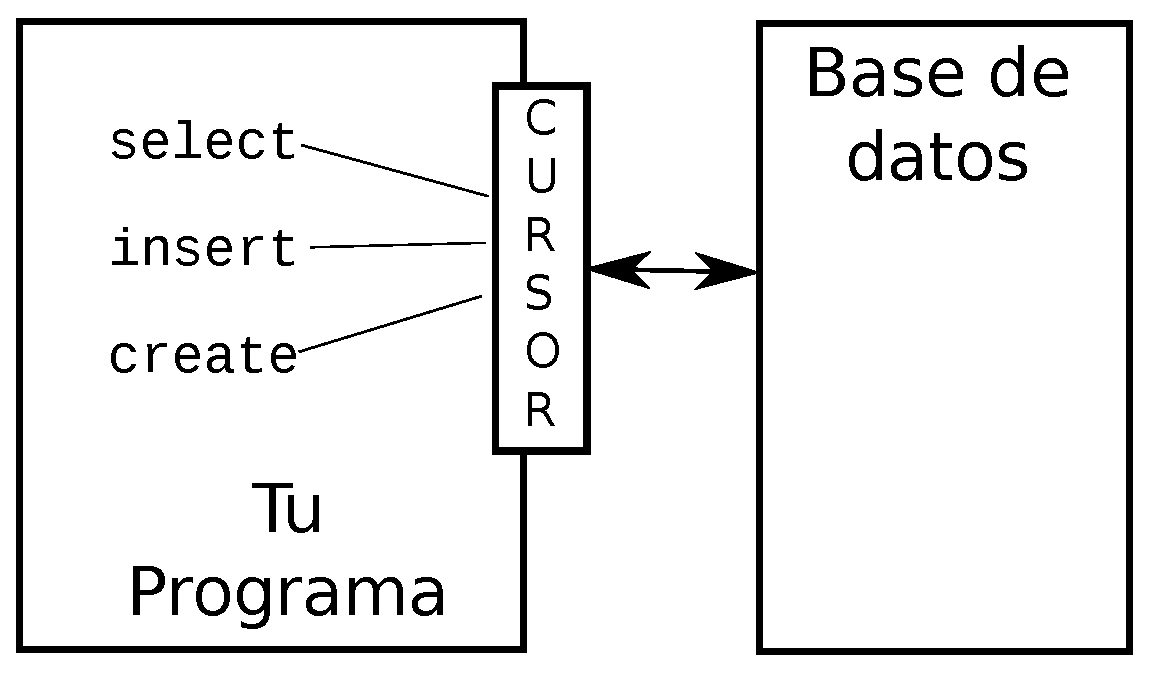
\includegraphics[height=1.50in]{figs2/cursor.eps}}
\afterfig

Una vez que tenemos el cursor, podemos comenzar a ejecutar
comandos sobre el contenido de la base de datos, usando el método
{\tt execute()}.

Los comandos de las bases de datos se expresan en un lenguaje especial que ha
sido estandarizado entre varios proveedores de bases de datos diferentes
para permitirnos aprender un único lenguaje para todas ellas. Este lenguaje
recibe el nombre de {\bf Lenguaje de Consultas eStructurado}, o {\bf SQL}
por sus iniciales en inglés.

\url{http://en.wikipedia.org/wiki/SQL}

En nuestro ejemplo, estamos ejecutando dos comandos SQL sobre la base de datos.
Por convención, mostraremos las palabras claves de SQL en mayúscula
y las partes de los comandos que añadamos nosotros (como los nombres
de las tablas y las columnas) irán en minúsculas.

El primer comando SQL elimina la tabla {\tt Canciones} de la
base de datos si ya existe. Este planteamiento se utiliza simplemente para permitirnos
ejecutar el mismo programa para crear la tabla {\tt Canciones} una y
otra vez sin provocar un error. Fíjate en que el comando
{\tt DROP TABLE} borra la tabla y todo su contenido
de la base de datos (es decir, aquí no existe la opción ``deshacer'').

\beforeverb
\begin{verbatim}
cur.execute('DROP TABLE IF EXISTS Canciones ')
\end{verbatim}
\afterverb
%
El segundo comando crea un tabla llamada
{\tt Canciones} con una columna de texto llamada {\tt titulo}
y una columna de enteros llamada {\tt reproducciones}.

\beforeverb
\begin{verbatim}
cur.execute('CREATE TABLE Canciones (titulo TEXT, reproducciones INTEGER)')
\end{verbatim}
\afterverb
%
Ahora que ya hemos creado la tabla llamada {\tt Canciones}, podemos guardar
algunos datos en ella usando la operación de SQL {\tt INSERT}. Empezaremos
realizando otra vez una conexión con la base de datos y obteniendo el {\tt cursor}.
Luego podremos ejecutar comandos SQL utilizando ese cursor.

El comando {\tt INSERT} de SQL indica qué tabla se está utilizando
y luego define una fila nueva, enumerando los campos que se desean
incluir {\tt (título, reproducciones)}, seguidos por los {\tt valores (VALUES)} que
se desean colocar en esa fila. Nosotros vamos a especificar los valores como signos de interrogación
{\tt (?, ?)} para indicarle que los valores reales serán pasados como una
tupla {\tt ( 'My Way', 15 ) } en el segundo parámetro de la
llamada a {\tt execute()}.

\beforeverb
\begin{verbatim}
import sqlite3

conn = sqlite3.connect('musica.sqlite3')
cur = conn.cursor()

cur.execute('INSERT INTO Canciones (titulo, reproducciones) VALUES ( ?, ? )', 
    ( 'Thunderstruck', 20 ) )
cur.execute('INSERT INTO Canciones (titulo, reproducciones) VALUES ( ?, ? )', 
    ( 'My Way', 15 ) )
conn.commit()

print 'Canciones:'
cur.execute('SELECT titulo, reproducciones FROM Canciones')
for fila in cur :
   print fila

cur.execute('DELETE FROM Canciones WHERE reproducciones < 100')
conn.commit()

cur.close()
\end{verbatim}
\afterverb
%
Primero {\tt insertamos (INSERT)} dos filas en la tabla y usamos {\tt commit()}
para forzar a que los datos sean escritos en el archivo de la base de datos.

\beforefig
\centerline{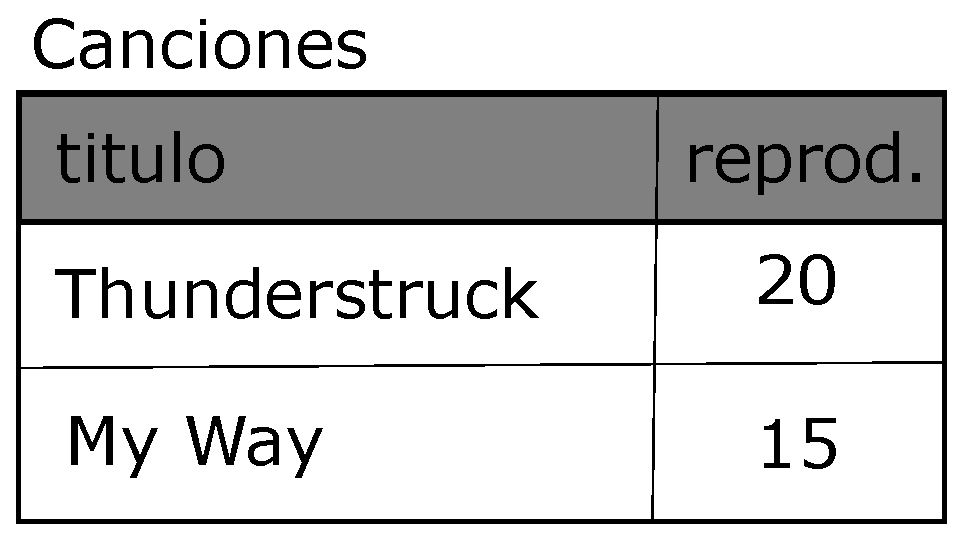
\includegraphics[height=1.00in]{figs2/tracks.eps}}
\afterfig

Después usamos el comando {\tt SELECT} para
recuperar las filas que acabamos de insertar en la tabla.
En el comando
{\tt SELECT}, indicamos qué columnas nos gustaría obtener {\tt (titulo, reproducciones)}
e indicamos desde qué tabla queremos recuperar los datos. Después de
ejecutar la sentencia {\tt SELECT}, el cursor se convierte en algo con lo que podemos
iterar mediante una sentencia {\tt for}. Por eficiencia,
el cursor no lee todos los datos de la base de datos
cuando se ejecuta la sentencia {\tt SELECT}.
En lugar de ello, los datos van siendo leídos según
se van pidiendo las filas desde el bucle creado con la sentencia {\tt for}.

La salida del programa es la siguiente:

\beforeverb
\begin{verbatim}
Canciones:
(u'Thunderstruck', 20)
(u'My Way', 15)
\end{verbatim}
\afterverb
%
\index{Unicode}
Nuestro bucle {\tt for} encuentra dos filas, y cada fila es una tupla de Python cuyo
primer valor es el {\tt título} y el segundo es el número de {\tt reproducciones}.
No nos preocupa que la cadena del título comience por
{\tt u'}. Se trata de una indicación de que las cadenas son del tipo {\bf Unicode},
y por tanto capaces de almacenar conjuntos de caracteres no-latinos.

Al final del programa, ejecutamos un comando SQL para {\tt borrar (DELETE)}
las filas que acabamos de crear, de modo que podamos ejecutar el programa una y otra vez.
El comando {\tt DELETE} nos muestra el uso de la cláusula {\tt WHERE}, la cual
nos permite expresar un criterio de selección, de modo que podemos pedir a la base de datos
que aplique el comando solamente a las filas que cumplan ese criterio. En este ejemplo,
el criterio es cumplido por todas las filas, así que vaciamos la tabla
para que podamos ejecutar el programa de nuevo repetidamente. Después de que se ha realizado el
{\tt DELETE}, llamamos de nuevo a {\tt commit()} para forzar a los datos a ser eliminados de
la base de datos.

\section{Resumen de Lenguaje de Consultas Estructurado}

Hasta ahora, hemos estado usando el Lenguaje de Consultas Estructurado en nuestros
ejemplos de Python y hemos utilizado muchos de los comandos básicos de SQL.
En esta sección, nos centraremos en el lenguaje SQL en particular
y echaremos un vistazo a su sintaxis.

A pesar de que hay muchos proveedores de bases de datos, el Lenguaje de Consultas
eStructurado (SQL) está estandarizado, de modo que podríamos comunicarnos de una forma
similar con sistemas de bases de datos de múltiples vendedores. 

Una base de datos relacional está compuesta por tablas, filas y columnas. Las columnas
tienen generalmente un tipo de datos que puede ser texto, numérico, o fecha. Cuando se crea
una tabla, se indican los nombres y tipos de cada columna.

\beforeverb
\begin{verbatim}
CREATE TABLE Canciones (titulo TEXT, reproducciones INTEGER)
\end{verbatim}
\afterverb
%
Para insertar una fila en una tabla, usamos el comando de SQL {\tt INSERT}:

\beforeverb
\begin{verbatim}
INSERT INTO Canciones (titulo, reproducciones) VALUES ('My Way', 15)
\end{verbatim}
\afterverb
%
La sentencia {\tt INSERT} especifica el nombre de la tabla, seguido por una lista
de los campos/columnas que se quieren establecer en la fila nueva, a continuación
la palabra clave {\tt VALUES} y una lista de los valores correspondientes
para cada uno de los campos.

El comando de SQL {\tt SELECT} se usa para recuperar filas y columnas desde una base de datos.
La sentencia {\tt SELECT} permite especificar qué columnas se quieren
recibir, junto con una clausula {\tt WHERE} para indicar qué 
filas se desean obtener. También permite una clausula opcional,
{\tt ORDER BY} para controlar el orden de las filas devueltas.

\beforeverb
\begin{verbatim}
SELECT * FROM Canciones WHERE titulo = 'My Way'
\end{verbatim}
\afterverb
%
El \verb"*" indica que se desea que la base de datos devuelva todas las
columnas para cada línea que cumpla la condición de la clausula {\tt WHERE}.

Fíjate que, a diferencia de lo que ocurre en Python, en SQL la clausula {\tt WHERE}
utiliza un único signo igual
para indicar una comprobación de igualdad, en lugar de utilizar un signo doble igual.
Otras operaciones lógicas que se permiten en una clausula {\tt WHERE} son
\verb"<",
\verb">",
\verb"<=",
\verb">=",
\verb"!=",
junto con {\tt AND}, {\tt OR} y paréntesis
para construir expresiones lógicas.

Se puede solicitar que las columnas devueltas vengan ordenadas por uno
de los campos así:

\beforeverb
\begin{verbatim}
SELECT titulo, reproducciones FROM Canciones ORDER BY titulo
\end{verbatim}
\afterverb
%
Para eliminar una fila, es necesario usar una clausula {\tt WHERE} en una sentencia
{\tt DELETE} de SQL. La clausula {\tt WHERE} determina qué filas serán eliminadas:

\beforeverb
\begin{verbatim}
DELETE FROM Canciones WHERE titulo = 'My Way'
\end{verbatim}
\afterverb
%
Es posible {\tt actualizar (UPDATE)} una columna o varias de una o más filas
en una tabla usando la sentencia de SQL {\tt UPDATE}, como se muestra a continuación:

\beforeverb
\begin{verbatim}
UPDATE Canciones SET reproducciones = 16 WHERE titulo = 'My Way'
\end{verbatim}
\afterverb
%
La sentencia {\tt UPDATE} especifica una tabla y a continuación
una lista de campos y valores a cambiar detrás de la palabra
clave {\tt SET}, y finalmente una clausula opcional {\tt WHERE} para elegir
las filas que van a ser actualizadas. Una única sentencia {\tt UPDATE}
cambiará todas las filas que coincidan con la clausula {\tt WHERE}.
Si no se ha especificado ninguna clausula {\tt WHERE}, se realizará la
{\tt actualización} de todas las filas de la tabla.

Existen cuatro comandos básicos de SQL (INSERT, SELECT, UPDATE y DELETE), que
nos permiten realizar las cuatro operaciones básicas necesarias para crear y mantener datos.

\section{Rastreo en Twitter usando una base de datos}

En esta sección, crearemos un programa araña sencillo que se moverá
a través de cuentas de Twitter y construirá una base de datos de ellas.
\emph{Nota: Ten mucho cuidado al ejecutar este programa. Si extraes
demasiados datos o ejecutas el programa durante demasiado tiempo
pueden terminar cortándote el acceso a Twitter.}

Uno de los problemas de cualquier tipo de programa araña es que se
necesita poderlo detener y volver a poner en marcha muchas veces, y
no se quieren perder los datos que se hayan recuperado hasta ese momento.
No querrás tener que empezar siempre la recuperación de datos desde
el principio, de modo que necesitaremos almacenar los datos según los vamos recuperando para
que nuestro programa pueda usar esa copia de seguridad y continuar de nuevo su recogida de datos
donde lo dejó la última vez.

Empezaremos por recuperar los amigos de Twitter de una persona y sus estados,
moviéndonos a través de la lista de amigos y añadiendo cada uno de ellos
a la base de datos para poder recuperarlos en el futuro. Después
de haber procesado todos los amigos de esa persona, consultaremos la base de datos
y recuperaremos los amigos de uno de esos amigos. Continuaremos haciendo esto una y otra vez,
recogiendo cualquier persona ``no visitada'', recuperando su lista de amigos
y añadiendo aquellos que no tengamos ya en nuestra lista para una próxima visita.

También rastrearemos cuántas veces hemos visto un amigo concreto en la
base de datos para tener una idea de su ``popularidad''.

Como estamos almacenando nuestra lista de cuentas de conocidos,
cuándo hemos recuperado una cuenta o no
y la popularidad de cada cuenta
en una base datos en el disco del ordenador,
podremos detener y reanudar el programa tantas veces como queramos. 

% POR HACER: Añadir una referencia al lugar correcto
Este programa es un poco complejo. Está basado en el código
de un ejercicio anterior del libro que usa la
API de Twitter.

Aquí está el código fuente para nuestra aplicación araña de Twitter:

\beforeverb
\begin{verbatim}
import urllib
import twurl
import json
import sqlite3

TWITTER_URL = 'https://api.twitter.com/1.1/friends/list.json'

conn = sqlite3.connect('arana.sqlite3')
cur = conn.cursor()

cur.execute('''
CREATE TABLE IF NOT EXISTS Twitter 
(nombre TEXT, recuperado INTEGER, amigos INTEGER)''')

while True:
    cuenta = raw_input('Introduce una cuenta de Twitter o salir: ')
    if ( cuenta == 'salir' ) : break
    if ( len(cuenta) < 1 ) :
        cur.execute('SELECT nombre FROM Twitter WHERE recuperado = 0 LIMIT 1')
        try:
            cuenta = cur.fetchone()[0]
        except:
            print 'No se han encontrado cuentas de Twitter por recuperar'
            continue

    url = twurl.augment(TWITTER_URL, 
               {'screen_name': cuenta, 'count': '20'} )
    print 'Recuperando', url
    conexion = urllib.urlopen(url)
    datos = conexion.read()
    cabeceras = conexion.info().dict
    # print 'Restante', cabeceras['x-rate-limit-remaining']
    js = json.loads(data)
    # print json.dumps(js, indent=4)

    cur.execute('UPDATE Twitter SET recuperado=1 WHERE nombre = ?', (cuenta, ) )

    contnuevas = 0
    contantiguas = 0
    for u in js['users'] :
        amigo = u['screen_name']
        print amigo
        cur.execute('SELECT amigos FROM Twitter WHERE nombre = ? LIMIT 1', 
            (amigo, ) )
        try:
            contador = cur.fetchone()[0]
            cur.execute('UPDATE Twitter SET amigos = ? WHERE nombre = ?', 
                (contador+1, amigo) )
            contantiguas = contantiguas + 1
        except:
            cur.execute('''INSERT INTO Twitter (nombre, recuperado, amigos) 
                VALUES ( ?, 0, 1 )''', ( amigo, ) )
            contnuevas = contnuevas + 1
    print 'Cuentas nuevas=',contnuevas,' ya visitadas=',contantiguas
    conn.commit()

cur.close()
\end{verbatim}
\afterverb
%
Nuestra base de datos está almacenada en el archivo {\tt arana.sqlite3} y tiene
una tabla llamada {\tt Twitter}. Cada fila en la tabla {\tt Twitter}
contiene una columna para el nombre de la cuenta, otra para indicar si hemos recuperado los
amigos de esa cuenta, y otra para guardar cuántas veces se ha visto esa cuenta añadida en
la lista de amigos de las demás.

En el bucle principal del programa, pedimos al usuario el nombre de una cuenta
de Twitter o ``salir'' para finalizar el programa.
Si el usuario introduce una cuenta de Twitter, recuperamos la
lista de amigos de ese usuario y sus estados,
y añadimos cada amigo a la base de datos si no
estaba ya en ella. Si el amigo ya está en la lista,
aumentamos en 1 el campo {\tt amigos} en la fila de la base de datos correspondiente.

Si el usuario pulsa intro, buscamos en la base de datos la siguiente
cuenta de Twitter que no haya sido aún recuperada, recuperamos los
amigos de esa cuenta y sus estados, y luego los añadimos a la base de datos
o los actualizamos, e incrementamos su contador de {\tt amigos}.

Una vez hemos recuperado la lista de amigos y sus estados, nos movemos
a través de los elementos {\tt users} del JSON devuelto
y recuperamos el \verb"screen_name" (nombre a mostrar) de cada usuario. Luego usamos
la sentencia {\tt SELECT} para comprobar si ya tenemos almacenado ese
nombre concreto en la base de datos y si es así recuperamos su
contador de amigos ({\tt amigos}).

\beforeverb
\begin{verbatim}
    contnuevas = 0
    contantiguas = 0
    for u in js['users'] :
	    amigo = u['screen_name']
	    print amigo
	    cur.execute('SELECT amigos FROM Twitter WHERE nombre = ? LIMIT 1', 
		    (amigo, ) )
	    try:
		    contador = cur.fetchone()[0]
		    cur.execute('UPDATE Twitter SET amigos = ? WHERE nombre = ?', 
			    (contador+1, amigo) )
		    contantiguas = contantiguas + 1
		except:
		    cur.execute('''INSERT INTO Twitter (nombre, recuperado, amigos) 
			    VALUES ( ?, 0, 1 )''', ( amigo, ) )
		    contnuevas = contnuevas + 1
    print 'Cuentas nuevas=',contnuevas,' ya visitadas=',contantiguas
    conn.commit()
\end{verbatim}
\afterverb
%
Una vez que el cursor ejecuta la sentencia {\tt SELECT},
debemos recuperar las filas. Podríamos hacerlo con una sentencia {\tt for},
pero dado que sólo estamos recuperando una única fila
({\tt LIMIT 1}), podemos también usar el método {\tt fetchone()} para extraer
la primera (y única) fila que da como resultado la operación {\tt SELECT}.
Dado que {\tt fetchone()} devuelve la fila como una {\bf tupla} (incluso si sólo
contiene un campo), tomamos el primer valor de la tupla mediante {\tt [0]}, para
almacenar así dentro de la variable {\tt contador} el valor del contador de amigos actual.

Si esta operación tiene éxito, usamos la sentencia {\tt UPDATE} de SQL con una
clausula {\tt WHERE} para añadir 1 a la columna {\tt amigos} de aquella fila que
coincida con la cuenta del amigo. Fíjate que hay dos marcadores de posición (es decir,
signos de interrogación) en el SQL, y que el segundo parámetro de {\tt execute()} es
una tupla de dos elementos que contiene los valores que serán sustituidos por esas
interrogaciones dentro de la sentencia SQL.

Si el código en el bloque {\tt try} falla, se deberá probablemente a que ningún registro
coincide con lo especificado en la clausula {\tt WHERE nombre = ?} de la sentencia SELECT.
Así que en el bloque {\tt except}, usamos la sentencia de SQL {\tt INSERT} para añadir el
nombre a mostrar (\verb"screen_name") del amigo a la tabla con una indicación de que no lo hemos
recuperado aún y fijamos su contador de amigos a cero.

La primera vez que el programa funciona e introducimos una cuenta de Twitter, mostrará
algo similar a esto:

\beforeverb
\begin{verbatim}
Introduce una cuenta de Twitter o salir: drchuck
Recuperando http://api.twitter.com/1.1/friends ...
Cuentas nuevas= 20  ya visitadas= 0
Introduce una cuenta de Twitter o salir: salir
\end{verbatim}
\afterverb
%
Dado que es la primera vez que ejecutamos el programa, la base de datos
está vacía, así que creamos el fichero {\tt arana.sqlite3} y añadimos
una tabla llamada {\tt Twitter} a la base de datos. A continuación
recuperamos algunos amigos y los añadimos a la base de datos, ya que
ésta está vacía.

En este momento, tal vez sea conveniente escribir un extractor de datos sencillo
para echar un vistazo a lo que hay dentro del fichero {\tt arana.sqlite3}:

\beforeverb
\begin{verbatim}
import sqlite3

conn = sqlite3.connect('arana.sqlite3')
cur = conn.cursor()
cur.execute('SELECT * FROM Twitter')
contador = 0
for fila in cur :
   print fila
   contador = contador + 1
print contador, 'filas.'
cur.close()
\end{verbatim}
\afterverb
%
Este programa simplemente abre la base de datos y selecciona todas las columnas
de todas las filas de la tabla {\tt Twitter}, luego
se mueve a través de las filas e imprime en pantalla su contenido.

Si lanzamos este programa después de la primera ejecución de nuestra araña
de Twitter, la salida que mostrará será similar a ésta:

\beforeverb
\begin{verbatim}
(u'opencontent', 0, 1)
(u'lhawthorn', 0, 1)
(u'steve_coppin', 0, 1)
(u'davidkocher', 0, 1)
(u'hrheingold', 0, 1)
...
20 filas.
\end{verbatim}
\afterverb
%
Vemos una fila para cada nombre, que aún no hemos
recuperado los datos de ninguno de esos nombres, y
que todo el mundo en la base de datos tiene un amigo.

En este momento la base de datos muestra la recuperación de los amigos de
nuestra primera cuenta de Twitter ({\bf drchuck}). Podemos ejecutar de nuevo
el programa y pedirle que recupere los amigos de la siguiente
cuenta ``sin procesar'', simplemente pulsando intro en vez de
escribir el nombre de una cuenta:

\beforeverb
\begin{verbatim}
Introduce una cuenta de Twitter o salir:  
Recuperando http://api.twitter.com/1.1/friends ...
Cuentas nuevas= 18  ya visitadas= 2
Introduce una cuenta de Twitter o salir: 
Recuperando http://api.twitter.com/1.1/friends ...
Cuentas nuevas= 17  ya visitadas= 3
Introduce una cuenta de Twitter o salir: salir
\end{verbatim}
\afterverb
%
Como hemos pulsado intro (es decir, no hemos especificado otra cuenta de Twitter),
se ha ejecutado el código siguiente:

\beforeverb
\begin{verbatim}
    if ( len(cuenta) < 1 ) :
        cur.execute('SELECT nombre FROM Twitter WHERE recuperado = 0 LIMIT 1')
        try:
            cuenta = cur.fetchone()[0]
        except:
            print 'No se han encontrado cuentas de Twitter por recuperar'
            continue
\end{verbatim}
\afterverb
%
Usamos la sentencia de SQL {\tt SELECT} para recuperar el nombre del primer
usuario ({\tt LIMIT 1}) que aún tiene su valor de ``hemos recuperado ya este usuario''
a cero. También usamos el modelo {\tt fechone()[0]} en un bloque
try/except para extraer el nombre de los datos recuperados o bien
mostrar un mensaje de error y volver al principio.

Si hemos recuperado con éxito el nombre de una cuenta que aún no había sido procesada,
tratamos sus datos de este modo:

\beforeverb
\begin{verbatim}
    url = twurl.augment(TWITTER_URL, {'screen_name': cuenta, 'count': '20'} )
    print 'Recuperando', url
    conexion = urllib.urlopen(url)
    datos = conexion.read()
    js = json.loads(datos)

    cur.execute('UPDATE Twitter SET recuperado=1 WHERE nombre = ?', (cuenta, ) )
\end{verbatim}
\afterverb
%
Una vez recuperamos los datos correctamente, usamos la sentencia {\tt UPDATE}
para poner la columna {\tt recuperado} a 1, lo que indica que hemos terminado
la recuperación de amigos de esa cuenta. Esto impide que recuperemos los
mismos datos una y otra vez y nos permite ir avanzando a través de la red
de amigos de Twitter. 

Si ejecutamos el programa de amigos y pulsamos intro dos veces para recuperar
los amigos del siguiente amigo no visitado,
y luego ejecutamos de nuevo el programa de extracción de datos, nos mostrará la
salida siguiente: 

\beforeverb
\begin{verbatim}
(u'opencontent', 1, 1)
(u'lhawthorn', 1, 1)
(u'steve_coppin', 0, 1)
(u'davidkocher', 0, 1)
(u'hrheingold', 0, 1)
...
(u'cnxorg', 0, 2)
(u'knoop', 0, 1)
(u'kthanos', 0, 2)
(u'LectureTools', 0, 1)
...
55 rows.
\end{verbatim}
\afterverb
%
Podemos ver que se han guardado correctamente las visitas que hemos realizado a
a {\tt lhawthorn} y {\tt opencontent}. Además las cuentas
{\tt cnxorg} y {\tt kthanos} ya tienen dos seguidores.
A pesar de hasta ahora hemos recuperados sólo los amigos de tres personas
({\tt drchuck}, {\tt opencontent}, y {\tt lhawthorn}), la tabla contiene ya
55 filas de amigos por recuperar.

Cada vez que ejecutamos el programa y pulsamos intro, se elegirá la siguiente
cuenta no visitada (es decir, ahora la siguiente cuenta sería \verb"steve_coppin"),
recuperará sus amigos, los marcará como recuperados, y para cada uno de los
amigos de \verb"steve_coppin" o bien lo añadirá al final de la
base de datos o bien actualizará su contador de amigos si ya estaba en la
tabla.

Como ves, al estar los datos del programa almacenados en el disco en una base de datos,
la actividad de rastreo puede ser suspendida y reanudada tantas veces como se desee
sin que se produzca ninguna pérdida de datos.

\section{Modelado de datos básico}

La potencia real de las bases de datos relacionales se manifiesta cuando se construyen múltiples
tablas y se crean enlaces entre ellas. El acto de decidir cómo separar los datos de tu
aplicación en múltiples tablas y establecer las relaciones
entre esas tablas recibe el nombre de {\bf modelado de datos}. El
documento de diseño que muestra las tablas y sus relaciones
se llama {\bf modelo de datos}.

El modelado de datos es una habilidad relativamente sofisticada, y en esta sección sólo
introduciremos los conceptos más básicos acerca de ello. Para obtener más
detalles sobre modelado de datos puedes comenzar con:

\url{http://en.wikipedia.org/wiki/Relational_model}

Supongamos que para nuestra aplicación de rastreo de Twitter, en vez de contar
los amigos de una persona sin más, queremos mantener una lista de
todas las relaciones entre ellos, de modo que podamos encontrar una lista de
gente que esté siguiendo la cuenta de una persona concreta.

Dado que todo el mundo puede tener potencialmente muchas cuentas siguiéndole,
no podemos añadir simplemente una única columna a nuestra tabla de {\tt Twitter}.
De modo que creamos una tabla nueva que realice un seguimiento de parejas de amigos.
A continuación se muestra un modo sencillo de hacer una tabla de este tipo:

\beforeverb
\begin{verbatim}
CREATE TABLE Camaradas (desde_amigo TEXT, hacia_amigo TEXT)
\end{verbatim}
\afterverb
%
Cada vez que encontremos a una persona de las que está siguiendo {\tt drchuck},
insertaremos una fila de esta forma:

\beforeverb
\begin{verbatim}
INSERT INTO Camaradas (desde_amigo, hacia_amigo) VALUES ('drchuck', 'lhawthorn')
\end{verbatim}
\afterverb
%
Según vayamos procesando los 20 amigos de {\tt drchuck}
que nos envía Twitter, insertaremos 20 registros con ``drchuck''
como primer parámetro, de modo que terminaremos duplicando la
cadena un montón de veces en la base de datos.

Esta duplicación de cadenas de datos viola una de las mejores prácticas
para la {\bf normalización de bases de datos}, que básicamente consiste en
que nunca se debe guardar la misma cadena de datos más de una vez en la base de datos.
Si se necesitan los datos varias veces, se debe crear una
{\bf clave} numérica para ellos y hacer referencia a los datos reales
a través de esa clave.

En términos prácticos, una cadena ocupa un montón
de espacio más que un entero, tanto en el disco como en
la memoria del ordenador, y además necesita más tiempo de procesador
para ser comparada y ordenada. Si sólo se tienen unos pocos cientos de entradas,
el espacio y el tiempo de procesador no importan demasiado. Pero si se tienen
un millón de personas en la base de datos y la posibilidad de 100 millones
de enlaces de amigos, es importante ser capaz de revisar los datos tan rápido
como sea posible.

Nosotros vamos a almacenar nuestras cuentas de Twitter en una tabla llamada {\tt Personas}
en vez de hacerlo en la tabla {\tt Twitter} que usamos en el ejemplo anterior.
La tabla {\tt Personas} tiene una columna adicional
para almacenar la clave numérica asociada con la
fila de cada usuario de Twitter.
SQLite tiene una característica que permite añadir automáticamente el valor de la clave
para cualquier fila que insertemos en la tabla, usando un tipo especial de
datos en la columna, ({\tt INTEGER PRIMARY KEY}).

Podemos, pues, crear la tabla {\tt Personas} con esa columna adicional
{\tt id}, como se muestra a continuación:

\beforeverb
\begin{verbatim}
CREATE TABLE Personas
    (id INTEGER PRIMARY KEY, nombre TEXT UNIQUE, recuperado INTEGER)
\end{verbatim}
\afterverb
%
Fíjate que ya no necesitamos mantener un contador de amigos en cada columna
de la tabla {\tt Personas}.
Cuando elegimos {\tt INTEGER PRIMARY KEY} como el tipo de la columna {\tt id},
estamos indicando que queremos que SQLite controle esta columna y
asigne automáticamente una clave numérica única para cada fila que insertemos.
También añadimos la palabra clave {\tt UNIQUE} para indicar que no vamos
a permitir a SQLite insertar dos filas con el mismo valor de {\tt nombre}.

Ahora en vez de crear la tabla {\tt Camaradas} como hicimos antes, crearemos
una tabla llamada {\tt Seguimientos} con dos columnas de tipo entero,
\verb"desde_id" y \verb"hacia_id", y una restricción en la tabla que consistirá en que
la \emph{combinación} de \verb"desde_id" y \verb"hacia_id" deberá ser única
(es decir, no se podrán insertar filas en la tabla con estos valores duplicados).

\beforeverb
\begin{verbatim}
CREATE TABLE Seguimientos 
    (desde_id INTEGER, hacia_id INTEGER, UNIQUE(desde_id, hacia_id) )
\end{verbatim}
\afterverb
%
Cuando añadimos la claúsula {\tt UNIQUE} a nuestras tablas, estamos comunicando un conjunto
de reglas que vamos a exigir a la base de datos que se cumplan cuando se intenten insertar
registros. Estamos creando esas reglas porque le convienen a nuestro programa, como
veremos dentro de un momento. Ambas reglas impiden que se cometan errores y hacen
más sencillo escribir parte de nuestro código.

En esencia, al crear esta tabla {\tt Seguimientos}, estamos modelando una
``relación'', en la cual una persona ``sigue'' a otra
y se representa con un par de números que indican que (a) ambas personas están
conectadas y (b) la dirección de la relación.

\beforefig
\centerline{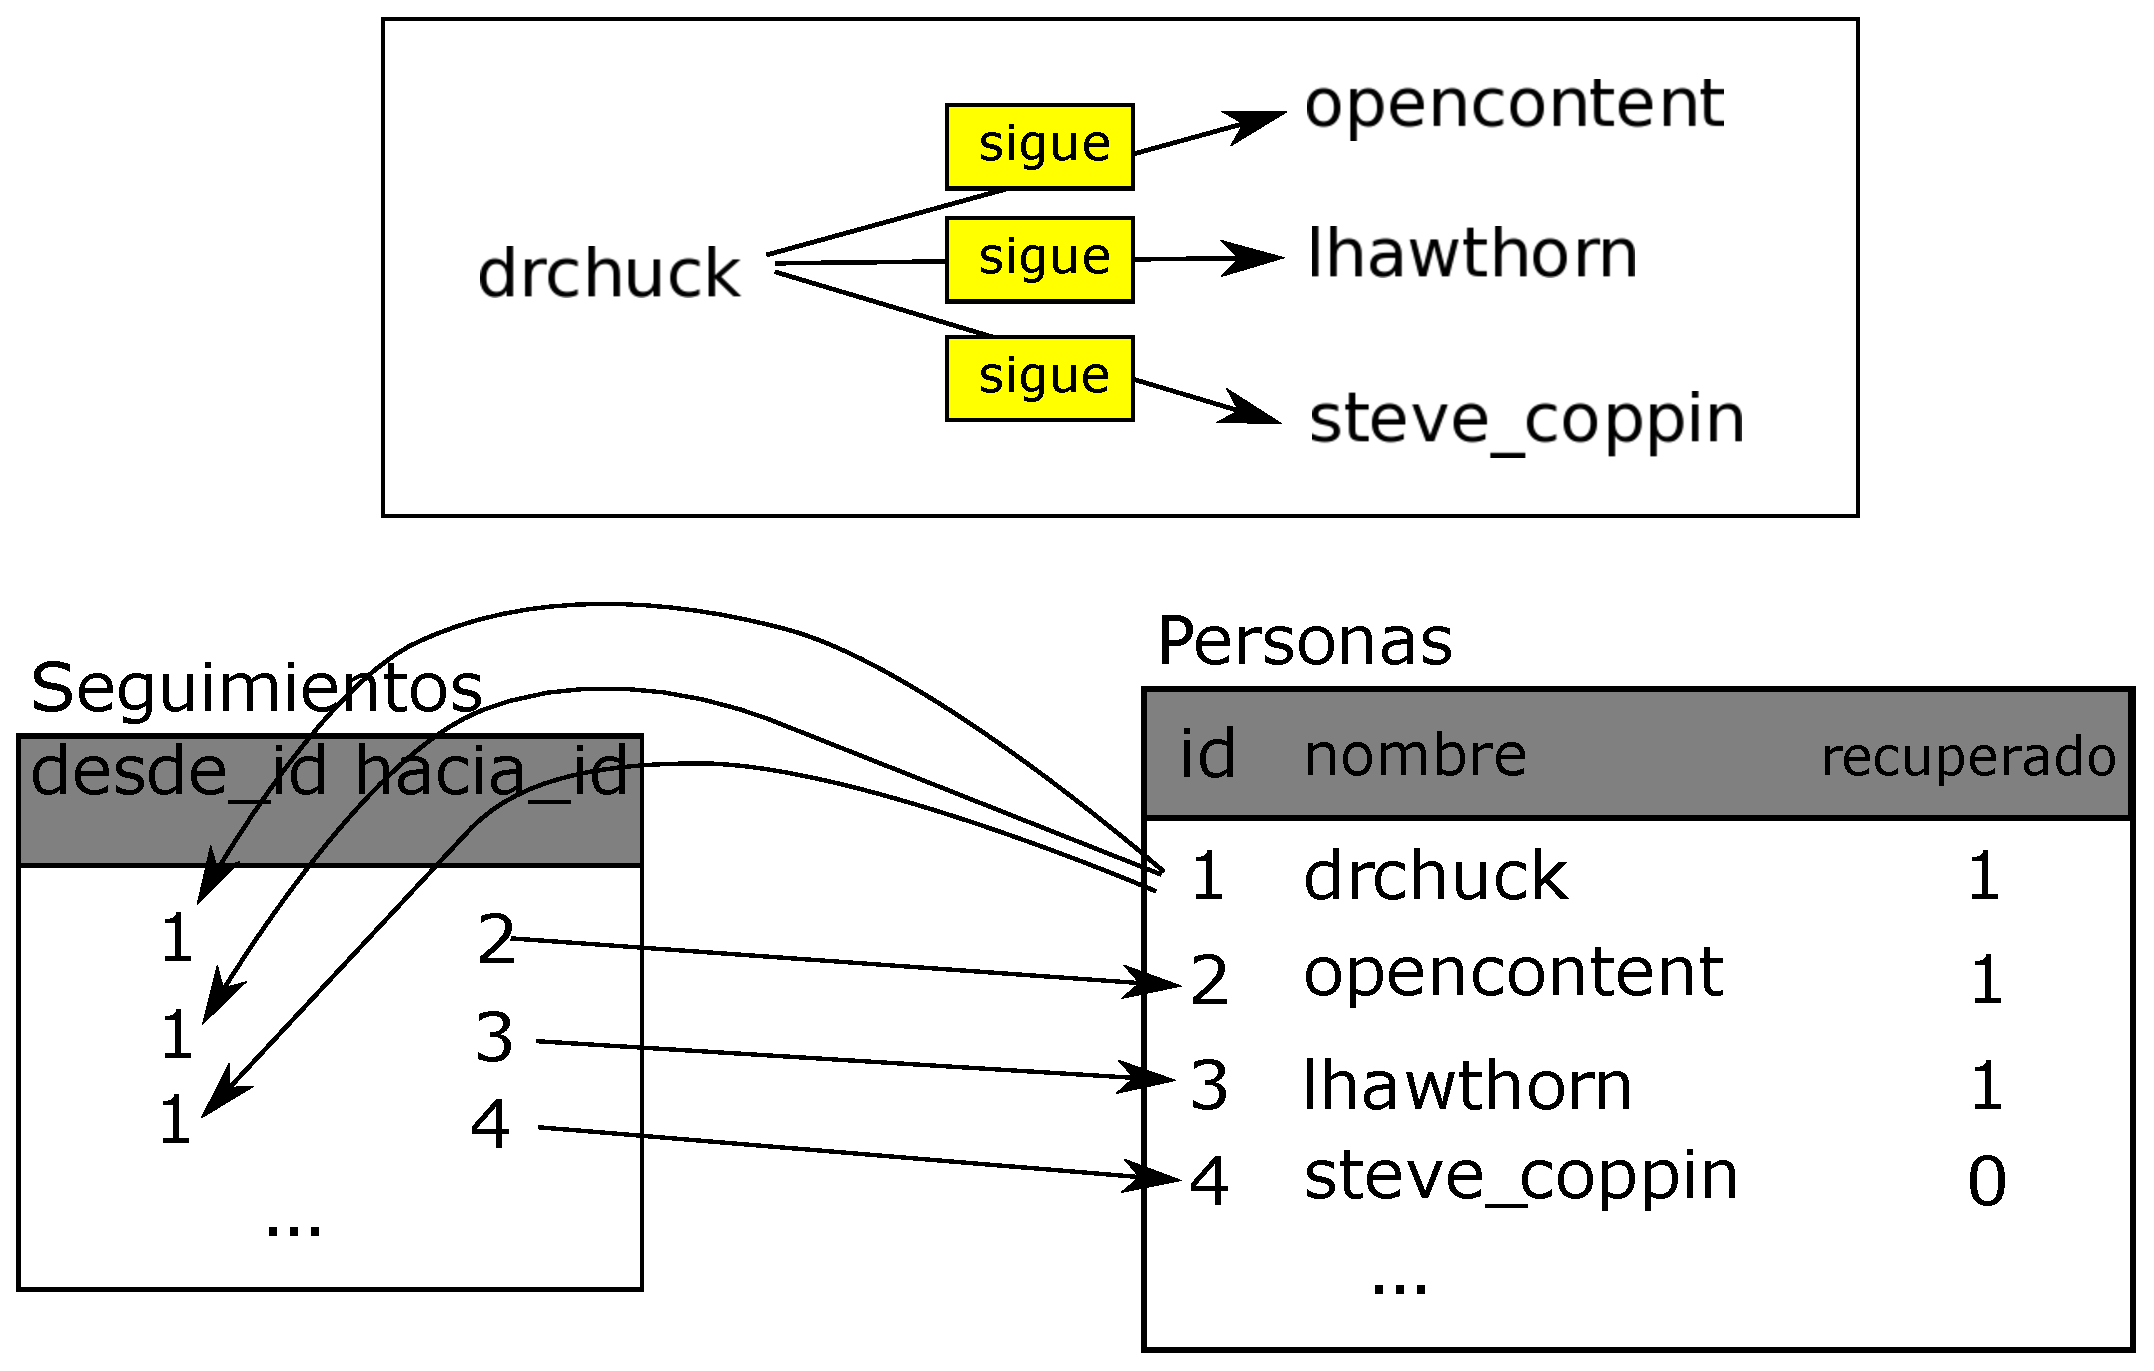
\includegraphics[height=2.50in]{figs2/twitter.eps}}
\afterfig


\section{Programación con múltiples tablas}

A continuación reharemos de nuevo el programa araña de Twitter usando dos tablas, las claves
primarias, y las claves de referencia, como hemos descrito antes. He aquí el código
de la nueva versión del programa:

\beforeverb
\begin{verbatim}
import urllib
import twurl
import json
import sqlite3

TWITTER_URL = 'https://api.twitter.com/1.1/friends/list.json'

conn = sqlite3.connect('amigos.sqlitesqlite3')
cur = conn.cursor()

cur.execute('''CREATE TABLE IF NOT EXISTS Personas 
    (id INTEGER PRIMARY KEY, nombre TEXT UNIQUE, recuperado INTEGER)''')
cur.execute('''CREATE TABLE IF NOT EXISTS Seguimientos 
    (desde_id INTEGER, hacia_id INTEGER, UNIQUE(desde_id, hacia_id))''')

while True:
    cuenta = raw_input('Introduce una cuenta de Twitter, o salir: ')
    if ( cuenta == 'salir' ) : break
    if ( len(cuenta) < 1 ) :
        cur.execute('''SELECT id, nombre FROM Personas
            WHERE recuperado = 0 LIMIT 1''')
        try:
            (id, cuenta) = cur.fetchone()
        except:
            print 'No se han encontrado cuentas de Twitter sin recuperar'
            continue
    else:
        cur.execute('SELECT id FROM Personas WHERE nombre = ? LIMIT 1', 
            (cuenta, ) )
        try:
            id = cur.fetchone()[0]
        except:
            cur.execute('''INSERT OR IGNORE INTO Personas (nombre, recuperado) 
                VALUES ( ?, 0)''', ( cuenta, ) )
            conn.commit()
            if cur.rowcount != 1 : 
                print 'Error insertando cuenta:',cuenta
                continue
            id = cur.lastrowid

    url = twurl.augment(TWITTER_URL, 
       {'screen_name': cuenta, 'count': '20'} )
    print 'Recuperando cuenta', cuenta
    conexion = urllib.urlopen(url)
    datos = conexion.read()
    cabeceras = conexion.info().dict
    print 'Restantes', cabeceras['x-rate-limit-remaining']

    js = json.loads(datos)
    # print json.dumps(js, indent=4)

    cur.execute('UPDATE Personas SET recuperado=1 WHERE nombre = ?', (cuenta, ) )

    contnuevas = 0
    contantiguas = 0
    for u in js['users'] :
        amigo = u['screen_name']
        print amigo
        cur.execute('SELECT id FROM Personas WHERE nombre = ? LIMIT 1', 
            (amigo, ) )
        try:
            amigo_id = cur.fetchone()[0]
            contantiguas = contantiguas + 1
        except:
            cur.execute('''INSERT OR IGNORE INTO Personas (nombre, recuperado) 
                VALUES ( ?, 0)''', ( amigo, ) )
            conn.commit()
            if cur.rowcount != 1 :
                print 'Error al insertar cuenta:',amigo
                continue
            amigo_id = cur.lastrowid
            contnuevas = contnuevas + 1
        cur.execute('''INSERT OR IGNORE INTO Seguimientos (desde_id, hacia_id) 
            VALUES (?, ?)''', (id, amigo_id) )
    print 'Cuentas nuevas=',contnuevas,' ya visitadas=',contantiguas
    conn.commit()

cur.close()
\end{verbatim}
\afterverb
%
Este programa empieza a resultar un poco complicado, pero ilustra
los patrones de diseño que debemos usar cuando utilizamos
claves de enteros para enlazar tablas. Esos patrones básicos son:

\begin{enumerate}

\item Crear tablas con claves primarias y restricciones.

\item Cuando tenemos una clave lógica para una persona (es decir, un
nombre de cuenta) y necesitamos el valor del {\tt id} de esa persona,
dependiendo de si esa persona ya está en la tabla
{\tt Personas} o no, tendremos que:
(1) buscar la persona en la tabla {\tt Personas} y
recuperar el valor de {\tt id} para esa persona,
o (2) añadir la persona a la tabla {\tt Personas} y obtener el
valor del {\tt id} para la fila recién añadida.

\item Insertar la fila que indica la relación de ``seguimiento''.

\end{enumerate}

Iremos explicando todos los puntos de uno en uno.

\subsection{Restricciones en tablas de bases de datos}

Una vez diseñada la estructura de la tabla, podemos indicar al sistema
de la base de datos que aplique unas cuantas reglas. Estas reglas nos
ayudarán a evitar errores y a introducir correctamente los datos en
las tablas. Cuando creemos nuestras tablas:

\beforeverb
\begin{verbatim}
cur.execute('''CREATE TABLE IF NOT EXISTS Personas 
    (id INTEGER PRIMARY KEY, nombre TEXT UNIQUE, recuperado INTEGER)''')
cur.execute('''CREATE TABLE IF NOT EXISTS Seguimientos 
    (desde_id INTEGER, hacia_id INTEGER, UNIQUE(desde_id, hacia_id))''')
\end{verbatim}
\afterverb
%
Estamos indicando que la columna {\tt nombre} de la tabla {\tt Personas} debe ser
{\tt UNIQUE} (única). Además indicamos que la combinación de los dos números
de cada fila de la tabla {\tt Seguimientos} debe ser también única. Estas restricciones
evitan que cometamos errores como añadir la misma relación entre las mismas personas
más de una vez.

Luego podemos aprovechar estas restricciones en el código siguiente:

\beforeverb
\begin{verbatim}
cur.execute('''INSERT OR IGNORE INTO Personas (nombre, recuperado) 
    VALUES ( ?, 0)''', ( amigo, ) )
\end{verbatim}
\afterverb
%
Aquí añadimos la clausula {\tt IGNORE} en la sentencia {\tt INSERT} para indicar
que si este {\tt INSERT} en concreto causara una violación de la regla
``el {\tt nombre} debe ser único'', el sistema de la base de datos está autorizado
a ignorar el {\tt INSERT}. De modo que estamos usando las restricciones de la base de datos
como una red de seguridad para asegurarnos de que no hacemos algo incorrecto de forma inadvertida.

De forma similar, el código siguiente se asegura de que no añadamos exactamente
la misma relación de {\tt Seguimiento} dos veces.

\beforeverb
\begin{verbatim}
cur.execute('''INSERT OR IGNORE INTO Seguimientos 
    (desde_id, hacia_id) VALUES (?, ?)''', (id, amigo_id) )
\end{verbatim}
\afterverb
%
Aquí también estamos simplemente indicándole a la base de datos que ignore cualquier intento
de {\tt INSERT} si éste viola la restricción de unicidad
que hemos especificado para cada fila de {\tt Seguimientos}.

\subsection{Recuperar y/o insertar un registro}

Cuando pedimos al usuario una cuenta de Twitter, si la cuenta ya
existe debemos buscar el valor de su {\tt id}. Si la cuenta
no existe aún en la tabla {\tt Personas}, debemos insertar
el registro y obtener el valor del {\tt id} de la fila
recién insertada.

Éste es un diseño muy habitual y se realiza dos veces en el programa anterior.
Este código muestra cómo se busca el {\tt id} de la
cuenta de un amigo, una vez extraído su \verb"screen_name"
desde un nodo de {\tt usuario} del JSON recuperado desde Twitter.

Dado que con el tiempo es probable que vayan aumentando las posibilidades de que la cuenta
ya figure en la base de datos, primero comprobamos si el registro
existe en {\tt Personas}, usando una sentencia {\tt SELECT}.

Si todo va bien\footnote{En general, cuando una frase comienza
``si todo va bien''	es porque el código del que se habla necesita
utilizar try/except.}, dentro de la sección {\tt try} recuperaremos el
registro mediante {\tt fetchone()} y luego recuperaremos el
primer (y único) elemento de la tupla devuelta, que almacenaremos en
\verb"amigo_id".

Si el {\tt SELECT} falla, el código {\tt fetchone()[0]} también fallará,
y el control será transferido a la sección {\tt except}.

\beforeverb
\begin{verbatim}
        amigo = u['screen_name']
        cur.execute('SELECT id FROM Personas WHERE nombre = ? LIMIT 1',
            (amigo, ) )
        try:
            amigo_id = cur.fetchone()[0]
            contantiguas = contantiguas + 1
        except:
            cur.execute('''INSERT OR IGNORE INTO Personas (nombre, recuperado) 
                VALUES ( ?, 0)''', ( amigo, ) )
            conn.commit()
            if cur.rowcount != 1 :
                print 'Error al insertar cuenta:',amigo
                continue
            amigo_id = cur.lastrowid
            contnuevas = contnuevas + 1
\end{verbatim}
\afterverb
%
Si terminamos en el código {\tt except}, eso sólo significa que la fila
no se ha encontrado en la tabla, de modo que deberemos insertarla. Usamos, pues,
{\tt INSERT OR IGNORE} sólo para evitar errores, y luego llamamos al {\tt commit()} para
forzar a la base de datos a que se actualice de verdad. Después de que se ha realizado la escritura,
ya podemos comprobar el {\tt cur.rowcount} para saber cuántas filas se han visto afectadas. Como
estamos intentando insertar una única fila, si el número de
filas afectadas es distinto de 1, se ha producido un error.

Si el {\tt INSERT} tiene éxito, podemos usar {\tt cur.lastrowid}
para averiguar el valor que la base de datos ha asignado a la columna {\tt id}
en nuestra fila recién creada.

\subsection{Almacenar las relaciones entre amigos}

Una vez que sabemos el valor de la clave tanto para del usuario de Twitter
como para el amigo que hemos extraído del JSON, resulta sencillo insertar
los dos números en la tabla de {\tt Seguimientos}
con el código siguiente:

\beforeverb
\begin{verbatim}
cur.execute('INSERT OR IGNORE INTO Seguimientos (desde_id, hacia_id) VALUES (?, ?)',
    (id, amigo_id) )
\end{verbatim}
\afterverb
%
Fíjate que dejamos que la base de datos se ocupe por nosotros de evitar la ``doble-inserción''
de una relación, mediante la creación de una tabla con una restricción de unicidad, de modo que
luego tan sólo añadimos {\tt o ignoramos} en nuestra sentencia {\tt INSERT}.

Una ejecución de ejemplo del programa sería la siguiente:

\beforeverb
\begin{verbatim}
Introduce una cuenta de Twitter, o salir:
No se han encontrado cuentas de Twitter sin recuperar
Introduce una cuenta de Twitter, o salir: drchuck
Recuperando http://api.twitter.com/1.1/friends ...
Cuentas nuevas= 20  ya visitadas= 0
Introduce una cuenta de Twitter, o salir: 
Recuperando http://api.twitter.com/1.1/friends ...
Cuentas nuevas= 17  ya visitadas= 3
Introduce una cuenta de Twitter, o salir:
Recuperando http://api.twitter.com/1.1/friends ...
Cuentas nuevas= 17  ya visitadas= 3
Introduce una cuenta de Twitter, o salir: salir
\end{verbatim}
\afterverb
%
Comenzamos con la cuenta de {\tt drchuck} y luego dejamos que el programa
escoja de forma automática las siguientes dos cuentas para recuperar y añadir
a nuestra base de datos.

Las siguientes son las primeras filas de las tablas {\tt Personas}
y {\tt Seguimientos} después de terminar la ejecución anterior:

\beforeverb
\begin{verbatim}
Personas:
(1, u'drchuck', 1)
(2, u'opencontent', 1)
(3, u'lhawthorn', 1)
(4, u'steve_coppin', 0)
(5, u'davidkocher', 0)
55 filas.
Seguimientos:
(1, 2)
(1, 3)
(1, 4)
(1, 5)
(1, 6)
60 filas.
\end{verbatim}
\afterverb
%
Puedes ver los campos {\tt id}, {\tt nombre}, y {\tt visitado} de la
tabla {\tt Personas}, y también los números de ambos extremos
de la relación en la tabla {\tt Seguidores}.
En la tabla {\tt Personas}, vemos que las primeras tres personas
han sido visitadas y que sus datos han sido recuperados.
Los datos de la tabla {\tt Seguidores} indican que
{\tt drchuck} (usuario 1) es amigo de todas las personas que se muestran en las primeras
cinco filas. Lo cual tiene sentido, porque
los primeros datos que hemos recuperado y almacenado fueron los amigos de Twitter de
{\tt drchuck}. Si imprimieras más filas de la tabla {\tt Seguimientos},
verías también los amigos de los usuarios 2 y 3.

\section{Tres tipos de claves}

Ahora que hemos empezado a construir un modelo de datos, colocando
nuestros datos en múltiples tablas enlazadas y hemos enlazado las filas de esas
tablas usando {\bf claves}, debemos fijarnos en cierta terminología
acerca de esas claves. Generalmente en un modelo de base de datos hay
tres tipos de claves que se pueden usar:

\begin{itemize}

\item Una {\bf clave lógica} es una clave que se podría usar en el ``mundo real''
para localizar una fila. En nuestro ejemplo de modelado de datos, el campo
{\tt nombre} es una clave lógica. Es el nombre que se muestra en pantalla para el usuario
y, en efecto, buscamos la columna de un usuario varias veces en el programa
usando el campo {\tt nombre}. A menudo verás que tiene sentido
añadir una restricción {\tt UNIQUE (única)} a una clave lógica. Ya que las
claves lógicas son las que usamos para buscar una fila desde el mundo exterior, tendría
poco sentido permitir que hubiera múltiples filas con el mismo valor en la tabla.

\item Una {\bf clave primaria} es normalmente un número que es asignado
automáticamente por la base de datos. En general no tiene ningún significado fuera
del programa y sólo se utiliza para enlazar entre si filas de tablas diferentes.
Cuando queramos buscar una fila en una tabla, realizar
la búsqueda usando la clave primaria es, normalmente, el modo
más rápido de localizarla. Como las claves primarias son números enteros,
necesitan muy poco espacio de almacenamiento y pueden ser comparadas u ordenadas muy rápido.
En nuestro modelo de datos, el campo {\tt id} es un ejemplo de una clave primaria.

\item Una {\bf clave foránea}\footnote{Se trata de una ``foreign key'', la cual se traduce
también a veces al español como ``clave extranjera'' (Nota del trad.)}
 es normalmente un número que apunta a la clave primaria
de una fila asociada en una tabla diferente. Un ejemplo de una clave foránea
en nuestro modelo de datos es la columna \verb"desde_id".

\end{itemize}

Estamos usando una
convención de nombres para darle siempre al campo de clave primaria el nombre
{\tt id} y añadir el sufijo \verb"_id" a cualquier nombre de campo
que sea una clave foránea.

\section{Uso de JSON para recuperar datos}

Ahora que hemos cumplido con las reglas de la normalización de bases de datos
y hemos separado los datos en dos tablas, enlazándolas entre sí usando
claves primarias y foráneas, necesitaremos ser capaces de construir un
{\tt SELECT} que vuelva a juntar los datos esparcidos por las tablas.

SQL usa la clausula {\tt JOIN} para volver a conectar esas tablas.
En la clausula {\tt JOIN} se especifican los campos que se utilizan
para reconectar las filas entre las distintas tablas.

A continuación se muestra un ejemplo de un {\tt SELECT} con una
clausula {\tt JOIN}:

\beforeverb
\begin{verbatim}
SELECT * FROM Seguimientos JOIN Personas 
    ON Seguimientos.desde_id = Personas.id WHERE Personas.id = 1
\end{verbatim}
\afterverb
%
La clausula {\tt JOIN} indica que los campos que estamos seleccionando
cruzan las tablas {\tt Seguimientos} y {\tt Personas}. La clausula
{\tt ON} indica cómo deben ser unidas las dos tablas: Toma cada fila
de {\tt Seguimientos} y añade una fila de {\tt Personas} en la cual el
campo \verb"desde_id" de {\tt Seguimientos} coincide con el valor {\tt id}
en la tabla {\tt Personas}.

\beforefig
\centerline{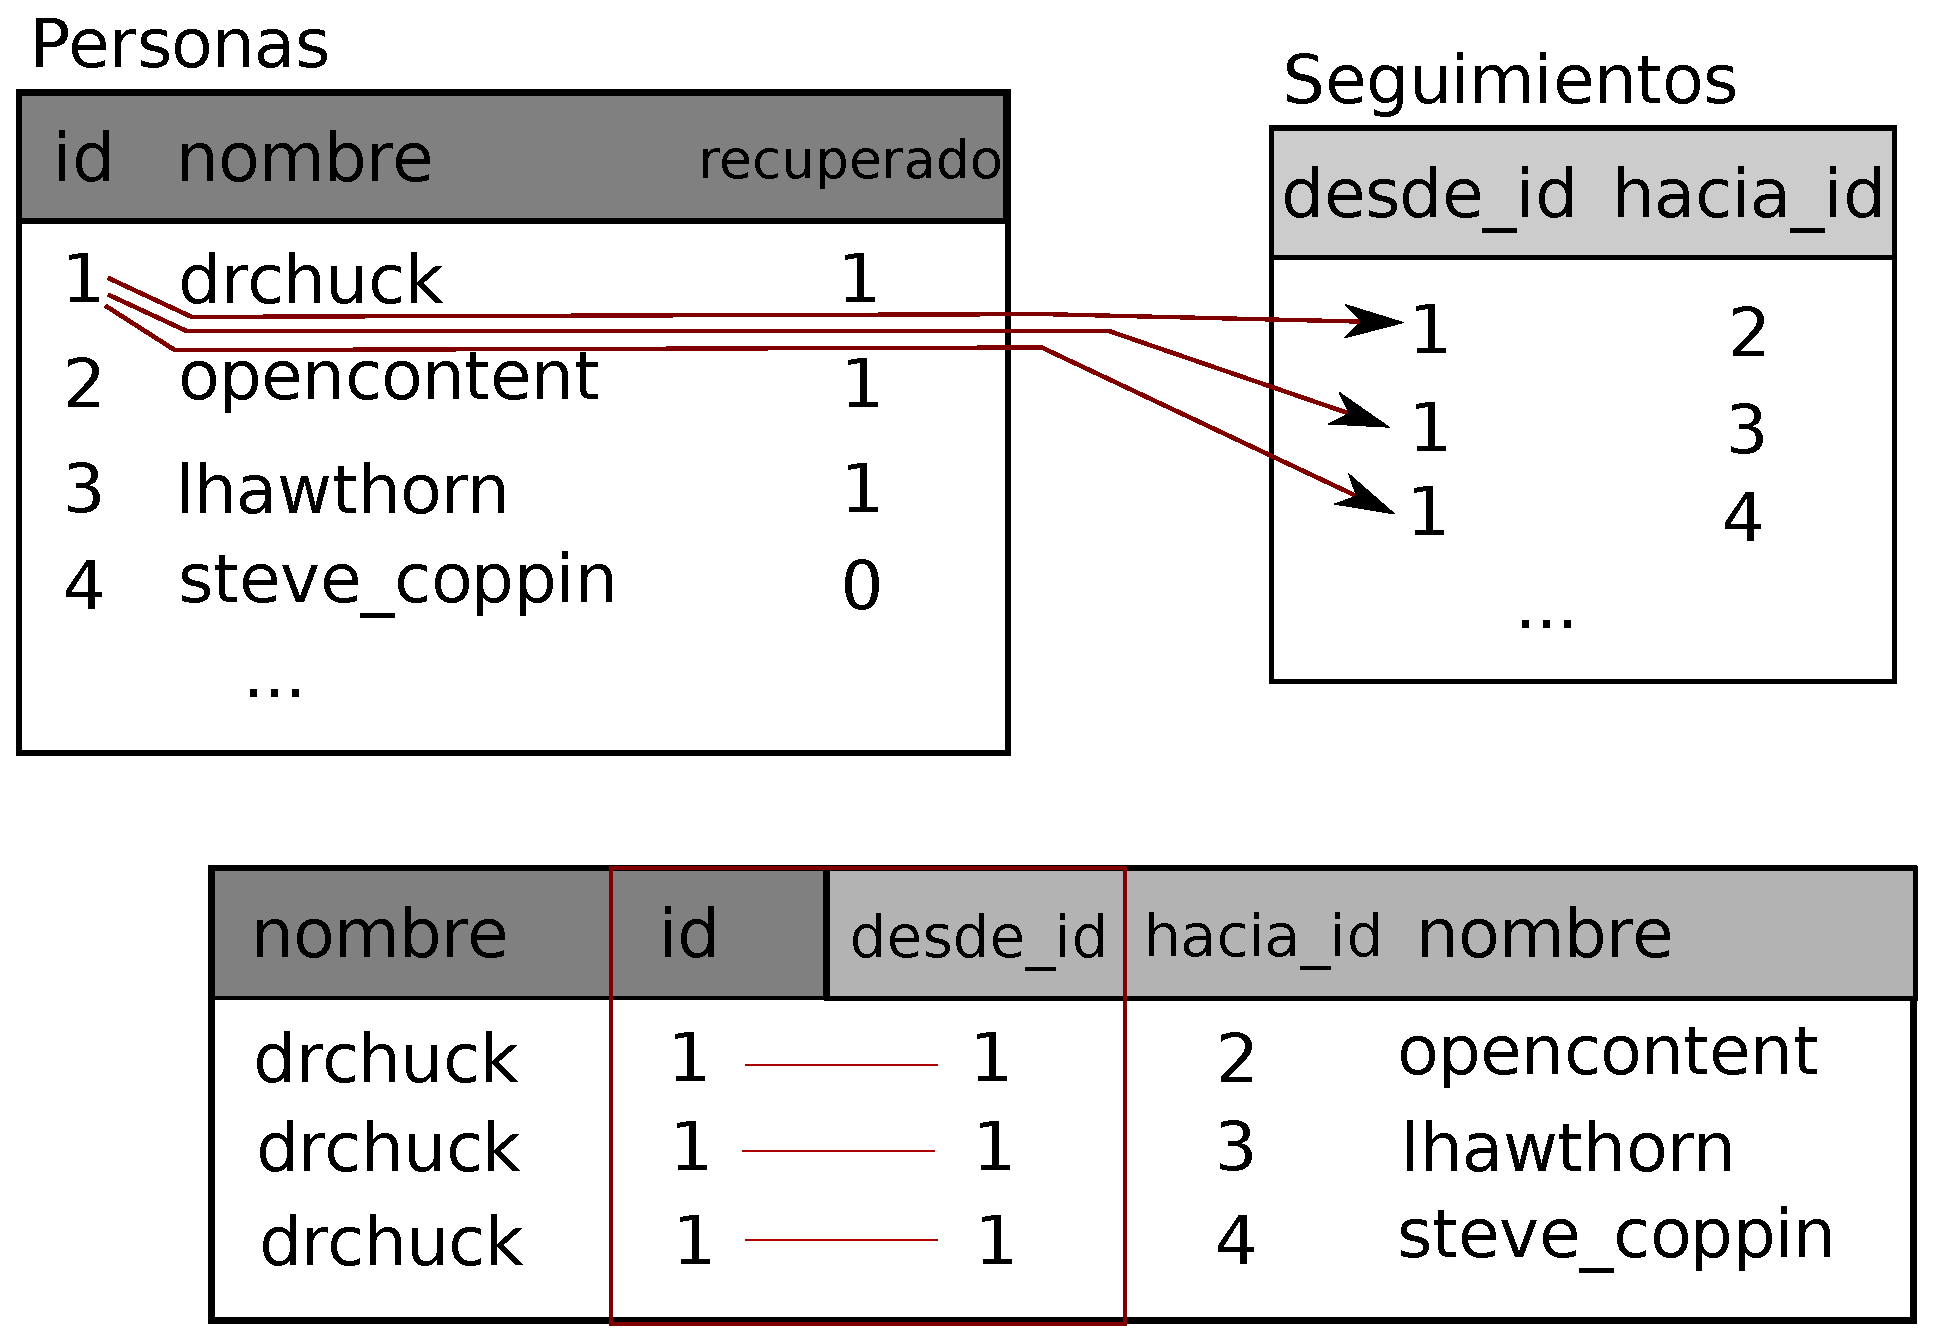
\includegraphics[height=2.50in]{figs2/join.eps}}
\afterfig

El resultado del JOIN consiste en la creación de una ``meta-fila'' extra larga, que contendrá
tanto los campos de {\tt Personas} como los campos de la fila de {\tt Seguimientos} que cumpla la
condición.
Cuando hay más de una coincidencia entre el campo {\tt id} de {\tt Personas}
y el \verb"desde_id" de {\tt Seguimientos}, JOIN creará una meta-fila
para \emph{cada una} de las parejas de filas que coincidan, duplicando los datos si es necesario.

El código siguiente muestra los datos que tendremos en la
base de datos después de que el programa multi-tabla araña de Twitter anterior
haya sido ejecutado varias veces.

\beforeverb
\begin{verbatim}
import sqlite3

conn = sqlite3.connect('arana.sqlite3')
cur = conn.cursor()

cur.execute('SELECT * FROM Personas')
contador = 0
print 'Personas:'
for fila in cur :
   if contador < 5: print fila
   contador = contador + 1
print contador, 'filas.'

cur.execute('SELECT * FROM Seguimientos')
contador = 0
print 'Seguimientos:'
for fila in cur :
   if contador < 5: print fila
   contador = contador + 1
print contador, 'filas.'

cur.execute('''SELECT * FROM Seguimientos JOIN Personas 
    ON Seguimientos.hacia_id = Personas.id WHERE Seguimientos.desde_id = 2''')
contador = 0
print 'Conexiones para id=2:'
for fila in cur :
   if contador < 5: print fila
   contador = contador + 1
print contador, 'filas.'

cur.close()
\end{verbatim}
\afterverb
%
En este programa, en primer lugar volcamos el contenido de las tablas {\tt Personas}
y {\tt Seguimientos} y a continuación mostramos un subconjunto de
datos de las tablas unidas entre sí.

Aquí tenemos la salida del programa:

\beforeverb
\begin{verbatim}
python twjoin.py 
Personas:
(1, u'drchuck', 1)
(2, u'opencontent', 1)
(3, u'lhawthorn', 1)
(4, u'steve_coppin', 0)
(5, u'davidkocher', 0)
55 filas.
Seguimientos:
(1, 2)
(1, 3)
(1, 4)
(1, 5)
(1, 6)
60 filas.
Conexiones para id=2:
(2, 1, 1, u'drchuck', 1)
(2, 28, 28, u'cnxorg', 0)
(2, 30, 30, u'kthanos', 0)
(2, 102, 102, u'SomethingGirl', 0)
(2, 103, 103, u'ja_Pac', 0)
20 filas.
\end{verbatim}
\afterverb
%
Se pueden ver las columnas de las tablas {\tt Personas} y {\tt Seguimientos}, seguidos del último
conjunto de filas, que es el resultado del {\tt SELECT} con la clausula {\tt JOIN}.

En el último select, buscamos las cuentas que sean amigas de
``opencontent'' (es decir, de {\tt Personas.id=2}).

En cada una de las ``meta-filas'' del último select, las primeras dos columnas pertenecen
a la tabla {\tt Seguimientos}, mientras que las columnas tres a cinco pertenecen a la tabla
{\tt Personas}. Se puede observar también cómo la segunda columna (\verb"Seguimientos.hacia_id")
coincide con la tercera ({\tt Personas.id}) en cada una de las ``meta-filas'' del join.

\section{Resumen}

En este capítulo se han tratado un montón de temas para darte una visión de conjunto del uso básico
de las bases de datos en Python. Es más complicado escribir el código para usar una base
de datos que almacene los datos que utilizar diccionarios de Python o archivos planos, de modo que
existen pocas razones para usar una base de datos a menos que tu aplicación necesite de verdad
las capacidades que proporciona. Las situaciones en las cuales una base de datos pueden resultar
bastante útil son:
(1) cuando tu aplicación necesita realizar muchos cambios pequeños de forma aleatoria en un conjunto
de datos grandes,
(2) cuando tienes tantos datos que no caben en un diccionario y necesitas localizar
información con frecuencia, o
(3) cuando tienes un proceso que va a funcionar durante mucho tiempo, y necesitas poder
detenerlo y volverlo a poner en marcha, conservando los datos entre ejecuciones.

Para cubrir las necesidades de muchas aplicaciones, una base de datos con una simple tabla puede
resultar suficiente, pero la mayoría de los problemas necesitarán varias tablas y enlaces/relaciones
entre filas de tablas diferentes. Cuando empieces a crear enlaces entre tablas,
es importante realizar un diseño meditado y seguir las
reglas de normalización de bases de datos para conseguir el mejor uso de sus capacidades.
Como la motivación principal para usar una base de datos
suele ser tener grandes cantidades de datos con las que tratar, resulta importante
modelar los datos de forma eficiente, de modo que tu programa funcione tan rápidamente como sea
posible. 

\section{Depuración}

Un enfoque común cuando se está desarrollando un programa en Python que conecte con
una base de datos SQLite será ejecutar primero el programa y revisar luego los
resultados usando el navegador de bases de datos de SQLite (SQLite Database Browser). El navegador
te permite revisar cuidadosamente los datos para comprobar si tu programa está funcionando
correctamente.

Debes tener cuidado, ya que SQLite se encarga de evitar que dos programa puedan
cambiar los mismos datos a la vez. Por ejemplo, si abres
una base de datos en el navegador y realizas un cambio en la base de datos,
pero no has pulsado aún el botón ``guardar'' del navegador, éste
``bloqueará'' el fichero de la base de datos y evitará que cualquier otro programa
acceda a dicho fichero. Concretamente, en ese caso tu programa Python
no será capaz de acceder al fichero si éste se encuentra bloqueado.

De modo que la solución pasa por asegurarse de cerrar el navegador de la base de datos,
o bien usar el menú {\bf Arhivo} para cerrar la base de datos abierta en el navegador
antes de intentar acceder a ella desde Python, para evitar encontrarse con
el problema de que el código de Python falle debido a que la base de datos
está bloqueada.

\section{Glosario}

\begin{description}

\item[atributo:] Uno de los valores dentro de una tupla. Más comúnmente
llamada ``columna'' o ``campo''..
\index{atributo}

\item[cursor:] Un cursor permite ejecutar comandos SQL en una base de datos
y recuperar los datos de ella. Un cursor es similar a un
socket en conexiones de red o a un manejador de ficheros.
\index{cursor}

\item[clave foránea:] Una clave numérica que apunta a la clave primaria de
una fila en otra tabla. Las claves foráneas establecen relaciones entre filas
almacenadas en tablas diferentes.
\index{foránea, clave}
\index{clave!foránea}

\item[clave lógica:] Una clave que el ``mundo exterior'' utiliza para localizar una fila
concreta. Por ejemplo, en una tabla de cuentas de usuario, la dirección de e-mail de una persona
sería un buen candidato a utilizar como clave lógica para los datos de ese usuario.
\index{lógica, clave}
\index{clave!lógica}

\item[clave primaria:] Una clave numérica asignada a cada fila que es utilizada para
referirnos a esa fila concreta de esa tabla desde otra tabla distinta. A menudo la base de datos
se configura para asignar las claves primarias de forma automática, según se van insertando filas.
\index{primaria, clave}
\index{clave!primaria}

\item[índice:] Datos adicionales que el software de la base de datos mantiene como filas
e inserta en una tabla para conseguir que las búsquedas sean muy rápidas.
\index{índice}

\item[navegador de base de datos:]
Un programa que permite conectar directamente con una base de datos
y manipularla, sin tener que escribir código para ello.
\index{gestor de bases de datos}
\index{base de datos!gestor}

\item[normalización:] Diseño de un modelado de datos de forma que no haya datos
duplicados. Se almacena cada elemento de los datos en un lugar concreto de la base de datos
y se referencia desde otros sitios usando una clave foránea.
\index{normalización}
\index{base de datos!normalización}

\item[relación:] Un área dentro de una base de datos que contiene tuplas y
atributos. Se la conoce más habitualmente como ``tabla''.
\index{relación}

\item[restricción:]
Cuando le pedimos a una base de datos que imponga una regla a una campo de una fila
en una tabla. Una restricción habitual consiste en especificar que no pueda haber
valores repetidos en un campo concreto (es decir, que todos los valores deban ser únicos). 
\index{restricción}

\item[tupla:] Una entrada única en una base de datos, que es un conjunto
de atributos. Se la conoce más habitualmente como ``fila''.
\index{tupla}

\end{description}